En esta parte de la investigación se presentan algunos antecedentes relacionados a la detección y pre-diagnóstico de nódulos en distintos órganos y a través de diversas metodologías. Estos ayudarán a entender el enfoque y obtener bases para un correcto desarrollo del proyecto en cuestión.

%% Primer antecedente : Deep-Learning-Based Morphological Feature Segmentation for Facial Skin Image Analysis
\subsection{\citetitle{yoon2023}}

\textbf{Introducción:}

El artículo \citetitle{yoon2023}, donde \cite{yoon2023} presentan un enfoque innovador para el análisis de imágenes faciales con el objetivo de segmentar características morfológicas de la piel, como arrugas y poros, utilizando una red neuronal profunda basada en U-Net. A diferencia de los métodos tradicionales que se enfocan en el color de la piel, este método utiliza estructuras morfológicas y se integra con mecanismos de atención y codificación posicional. Esto permite una detección simultánea más precisa de arrugas y poros, un avance significativo en el campo de la dermatología estética y la industria cosmética.

\textbf{Técnicas utilizadas:}

Para potenciar la capacidad de U-Net en la distinción de rasgos faciales morfológicos, los autores incorporan esquemas de atención en dos niveles: una atención espacial ubicada en el cuello de botella (\textit{bottleneck}) para recalcar regiones con alta probabilidad de contener arrugas o poros, y módulos de atención aditiva (\textit{Additive Attention Module}, AAM) en las conexiones de “skip” que aprenden a fusionar selectivamente las características del codificador (clave y valor) con la información contextual del decodificador (consulta). Este doble mecanismo no solo mejora la convergencia del modelo, sino que reduce significativamente los falsos positivos al impedir que zonas irrelevantes influyan en la predicción.

En cuanto a la generación de la \textit{ground truth}, se diseñaron dos mapas de textura, como se ve en la Figura \ref{2:figmapant1}:

\begin{itemize}
    \item \textbf{Mapa de textura para arrugas:} basado en un filtro que combina un suavizado Gaussiano y la comparación entre la intensidad original y su versión filtrada para realzar bordes continuos;
    \item \textbf{Mapa de textura para poros:} obtenido mediante pirámide Laplaciana, donde los niveles bajos ($L_0$ y $L_1$) se combinan y umbralizan para destacar las pequeñas discontinuidades que corresponden a los poros.
\end{itemize}

\begin{figure}[H]
	\begin{center}
		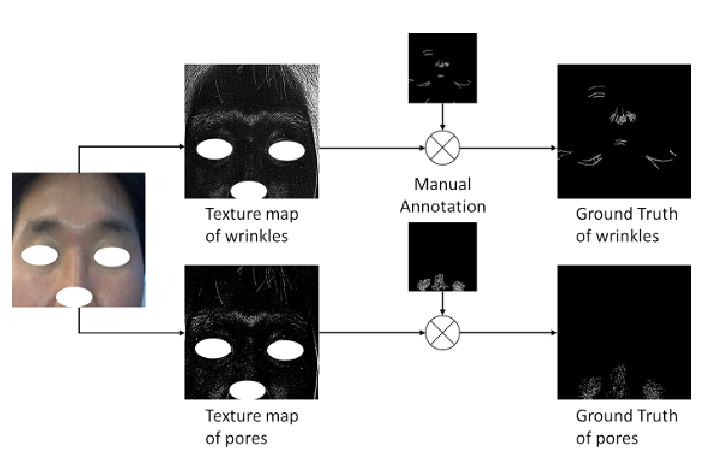
\includegraphics[width=0.75\textwidth]{2/figures/mapsant1.png}
		\caption[Mapas de textura para arrugas y poros]{Mapas de textura para arrugas y poros.\\
		Fuente: \cite{yoon2023}. \citetitle{yoon2023}. (p. 4)}
		\label{2:figmapant1}
	\end{center}
\end{figure}

Estas texturas, multiplicadas por anotaciones manuales gruesas, generan GT con contornos definidos y adaptados a la resolución de cada rasgo, facilitando el aprendizaje diferencial de líneas frente a puntos.

Finalmente, para incorporar información posicional, los autores aplican un \textit{padding} de ceros alrededor de la imagen original (\textit{zero-padding}), de modo que la red, al procesar imágenes de tamaño $(Z+H) \times (Z+W)$, internalice la posición predominante de arrugas (frente, contorno de ojos) y poros (zona “mariposa” de mejillas y nariz), reduciendo detecciones erróneas en regiones atípicas.

\textbf{Metodología:}
La metodología, como se puede ver en el diagrama creado en la Figura \ref{2:figant1}, sigue un flujo sistemático compuesto por cinco fases principales:

\begin{enumerate}[label=\textbf{\arabic*.}, leftmargin=2em]
    \item \textbf{Data Collection:} Se recolectaron 314 imágenes faciales mediante dispositivos especializados de diagnóstico de piel. Las imágenes capturaron regiones relevantes como frente, ojos y mejillas. Se obtuvo consentimiento informado de los participantes.
    \item \textbf{Data Preparation:} Las imágenes se recortaron y redimensionaron a $768 \times 640$ píxeles, aplicándoles \textit{zero-padding}. Se generaron anotaciones manuales refinadas con mapas de textura específicos para arrugas (filtros Gaussiano) y poros (pirámide Laplaciana).
    \item \textbf{Network Architecture Design:} Se diseñó un U-Net “reducido”, con atención espacial en el cuello de botella y módulos de atención aditiva (AAM) en las conexiones de salto, enfocándose en las zonas relevantes para arrugas y poros.
    \item \textbf{Model Training and Testing:} Se entrenó la red usando 264 imágenes para entrenamiento y 50 para validación, optimizando con MSE Loss. El entrenamiento se realizó en PyTorch utilizando una GPU RTX 3060.
    \item \textbf{Results and Evaluation:} Las predicciones se compararon con métodos de imagen clásicos y U-Net++. El modelo propuesto mejoró la segmentación, logrando un IoU de 0.2341 en arrugas y 0.4032 en poros, mostrando mayor precisión y reducción de falsos positivos gracias a los mecanismos de atención y codificación posicional.
\end{enumerate}

\begin{figure}[H]
	\begin{center}
		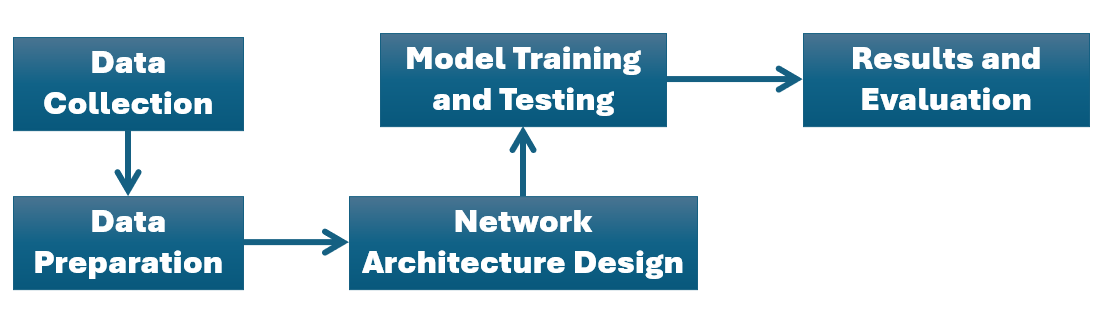
\includegraphics[width=1\textwidth]{2/figures/metoant1.png}
		\caption[Metodología propuesta por el primer antecedente]{Metodología propuesta por el primer antecedente.\\
			Fuente: Elaboración propia}
		\label{2:figant1}
	\end{center}
\end{figure}

\textbf{Base de datos utilizada:}
Aunque no se empleó un conjunto de datos público estandarizado, los autores recolectaron 314 imágenes faciales de alta resolución mediante sistemas de diagnóstico de piel (e.g., Lumini Kiosk V2). Tras recorte y escalado a 768×640, 264 imágenes sirvieron para entrenamiento y 50 para validación. Las anotaciones de GT partieron de “borradores” manuales que capturaban la extensión aproximada de arrugas y poros, pulidos mediante la aplicación de los mapas de textura generados automáticamente. Esta estrategia semiautomática redujo el tiempo de etiquetado y garantizó la coherencia en la forma y tamaño de los rasgos segmentados .

\textbf{Resultados:}
Los resultados, como se puede ver en la Tabla \ref{tab:models_performance} y en la Figura \ref{2:fig1}, demuestran una mejora global en la detección simultánea de arrugas y poros:

\begin{itemize}
    \item \textbf{Precisión espacial:} Las máscaras de segmentación reproducen con alta fidelidad la forma y localización de arrugas delgadas y gruesas, así como la distribución de poros, incluso en presencia de variaciones de iluminación.
    \item \textbf{Reducción de falsos positivos:} El uso de \textit{zero-padding} y mecanismos de atención reduce la detección en zonas atípicas (p. ej., líneas finas fuera de la región periocular detectadas por U-Net puro) y áreas de alta frecuencia que no corresponden a poros.
    \item \textbf{Métricas cuantitativas:} La mejora de IoU para poros (+10 \% respecto a U-Net++) y para arrugas (+8 \%) evidencia el aporte de cada componente metodológico (atención, GT semántico, \textit{padding}).
\end{itemize}

Además, el estudio de ablación muestra que un U-Net reducido con atención y \textit{zero-padding} (5.2 M parámetros) supera tanto al U-Net completo (17.3 M) como a U-Net++ en Loss e IoU, validando que el tamaño de la red puede optimizarse sin sacrificar rendimiento.


\begin{table}[H]
    \centering
    \caption{Métricas de rendimiento de diferentes modelos}
    \renewcommand{\arraystretch}{1.2} % Adjust row spacing
    \setlength{\tabcolsep}{5pt} % Adjust column spacing
    \begin{tabularx}{\textwidth}{@{}X c c c c@{}}
        \toprule
        \textbf{Models} & \textbf{\#Params} & \textbf{Loss} & \textbf{IoU of Wrinkle} & \textbf{IoU of Pore} \\ \midrule
        U-Net & 17.3 M & 1.243 & 0.2078 & 0.3601 \\
        Reduced U-Net & 4.3 M & 1.250 & 0.2147 & 0.3646 \\
        Reduced U-Net, Attentions & 5.2 M & 1.242 & 0.2250 & 0.3714 \\
        Reduced U-Net, Attentions, Zero-padding (Proposed) & 5.2 M & 1.145 & 0.2341 & 0.4032 \\ 
        \bottomrule
    \end{tabularx}
    \label{tab:models_performance}
\end{table}


\begin{figure}[H]
	\begin{center}
		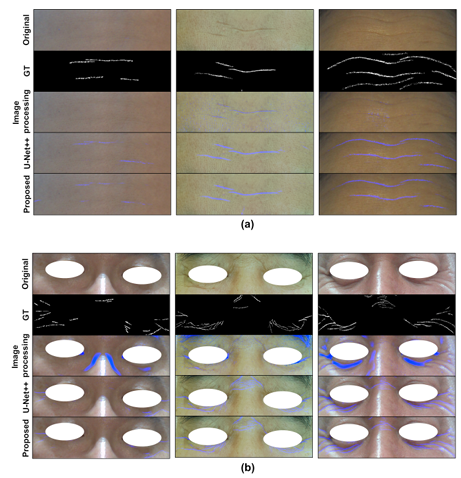
\includegraphics[width=0.75\textwidth]{2/figures/resant1.png}
		\caption[Comparación de la segmentación de arrugas en (a) la frente y (b) la región de los ojos]{Comparación de la segmentación de arrugas en (a) la frente y (b) la región de los ojos.\\
			Fuente: \cite{yoon2023}. \citetitle{yoon2023}. (p. 10)}
		\label{2:fig1}
	\end{center}
\end{figure}

\textbf{Conclusiones:}
\cite{yoon2023} presentan un método pionero para la segmentación simultánea de arrugas y poros en imágenes faciales, superando enfoques clásicos y recientes variantes de U-Net. La combinación de GT semiautomáticos basados en texturas, mecanismos de atención y codificación posicional produce un modelo compacto, preciso y robusto ante variaciones de iluminación y tipos de piel. Sus aplicaciones potenciales abarcan la estimación de edad facial, la predicción de enfermedades dermatológicas y el asesoramiento cosmético personalizado. Como direcciones futuras, los autores sugieren: integrar directamente la severidad de los rasgos en un único modelo end-to-end, mejorar la coherencia de las GT con postprocesamientos avanzados y explorar funciones de pérdida específicas (Dice, pérdidas ponderadas) para optimizar aún más la segmentación en escenarios con desequilibrio de clases .

%% Segundo antecedente :  High Performing Facial Skin Problem Diagnosis with Enhanced Mask R-CNN and Super Resolution GAN
\subsection{\citetitle{Kim2023}}

\textbf{Introducción:}
El artículo de \cite{Kim2023} titulado \citetitle{Kim2023}, aborda la importancia de un diagnóstico preciso de problemas faciales de la piel, que afectan aspectos como la percepción de edad, belleza y salud. Tradicionalmente, este diagnóstico requiere visitas a clínicas especializadas, lo cual es costoso y poco práctico. Como alternativa, se propone el uso de algoritmos de aprendizaje automático para realizar diagnósticos más accesibles. Sin embargo, los enfoques basados en redes neuronales convolucionales (CNN) enfrentan desafíos técnicos, como la dificultad para detectar problemas pequeños, la identificación de hasta 20 tipos diferentes de problemas cutáneos, y la segmentación incorrecta en áreas no faciales. El objetivo del estudio es superar estas limitaciones mediante cinco tácticas específicas.

\textbf{Técnicas utilizadas:}

Para afrontar los múltiples retos técnicos descritos, el estudio propone un enfoque combinado e innovador que integra:

\begin{itemize}
    \item \textbf{Enhanced Mask R-CNN:} Se trata de una versión refinada de la arquitectura Mask R-CNN, modificada específicamente para mejorar la segmentación de objetos de pequeño tamaño. Para lograrlo, se añaden capas de fusión y capas de deconvolución, lo que permite retener mejor los detalles finos en las imágenes faciales, como lo vemos en la Figura \ref{2:figant2rcnn}.
    \begin{figure}[H]
		\begin{center}
			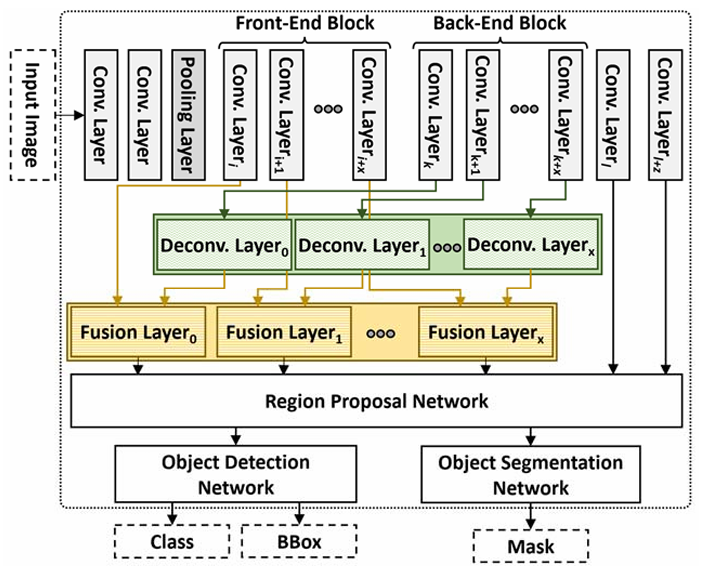
\includegraphics[width=0.75\textwidth]{2/figures/estant2.png}
			\caption[Estructura de la máscara refinada R-CNN para objetos de tamaño pequeño]{Estructura de la máscara refinada R-CNN para objetos de tamaño pequeño.\\
				Fuente: \cite{Kim2023}. \citetitle{Kim2023}. (p. 7)}
			\label{2:figant2rcnn}
		\end{center}
	\end{figure}
	\item \textbf{Super-Resolution Generative Adversarial Networks (SR-GAN):} Se utiliza esta técnica para mejorar la resolución y calidad de las imágenes de entrada. Al aplicar SR-GAN, se amplifican las áreas pequeñas y borrosas, permitiendo que los modelos de segmentación detecten detalles que normalmente pasarían desapercibidos, como lo vemos en la Figura \ref{2:figant2srgan}.
    \begin{figure}[H]
		\begin{center}
			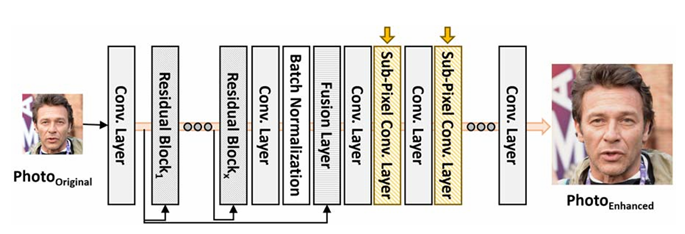
\includegraphics[width=0.75\textwidth]{2/figures/ant2srgan.png}
			\caption[Generador en SR-GAN con capas de convolución de subpíxeles]{Generador en SR-GAN con capas de convolución de subpíxeles.\\
				Fuente: \cite{Kim2023}. \citetitle{Kim2023}. (p. 7)}
			\label{2:figant2srgan}
		\end{center}
	\end{figure}
	\item \textbf{Ajustes de redes neuronales:} Se realizan ajustes de arquitectura específicos para mejorar el manejo de objetos pequeños y para reducir errores de segmentación en áreas no relevantes (como el cabello o el fondo de la foto).
    \item \textbf{Mejoras en la diferenciación de problemas similares:} Se incorporan técnicas para distinguir visualmente problemas de piel que presentan alta similitud (como manchas de hiperpigmentación y lunares), aumentando la precisión diagnóstica.
    \item \textbf{Mecanismos de limpieza de predicciones:} Se diseñan procedimientos de post-procesamiento que eliminan falsas segmentaciones basadas en el reconocimiento de \textit{landmarks} faciales, garantizando que sólo se conserven segmentaciones realizadas dentro de las zonas faciales válidas.
\end{itemize}

Cada una de estas técnicas fue meticulosamente desarrollada e integrada en un flujo de procesamiento automático, garantizando una mejora sustancial sobre las técnicas tradicionales de diagnóstico basadas en CNN.

\textbf{Metodología:}
La metodología general del artículo se articula en cinco fases principales, reflejadas en la Figura \ref{2:figant2}, diseñadas para abordar los desafíos identificados:


\begin{enumerate}[label=\textbf{\arabic*.}, leftmargin=2em]
    \item \textbf{Refining Mask R-CNN Network with Fusion and Deconvolution Layers}
	La primera táctica consistió en modificar la arquitectura convencional de Mask R-CNN para mejorar su desempeño en la detección de problemas cutáneos de pequeño tamaño. Para ello:
	
	\begin{itemize}
		\item Se diseñaron capas de fusión que integran información de diferentes niveles de profundidad de la red, combinando características de alto nivel semántico con detalles de baja escala.
		\item Se añadieron capas de deconvolución que permiten reconstruir información espacial de alta resolución a partir de mapas de características comprimidos.
	\end{itemize}
	Esta mejora en la arquitectura favorece una segmentación más precisa de detalles pequeños como poros, arrugas finas o pequeñas manchas, cuya detección era limitada en enfoques CNN tradicionales.
	
	\item \textbf{Super Resolution GAN for Small-sized and Blurry Images}
	La segunda táctica introdujo el uso de SR-GAN para la mejora de calidad de las imágenes de entrada. Específicamente:
	
	\begin{itemize}
		\item Se aplicó un modelo GAN especializado en super-resolución para ampliar las regiones de interés en las imágenes.
		\item Esta técnica permitió mejorar la nitidez y resolución de pequeñas lesiones cutáneas, haciendo que las redes segmentadoras pudieran capturar más detalles y aumentar su precisión.
		\item El generador de SR-GAN utiliza capas de convolución sub-pixel para reconstruir imágenes de alta calidad a partir de datos de baja resolución.
	\end{itemize}
	
	\item \textbf{Training Facial Skin Problem-specific Segmentation Models}
	En la tercera fase se entrenaron modelos de segmentación especializados en un único tipo de problema cutáneo:
	
	\begin{itemize}
		\item En lugar de entrenar un modelo general para reconocer múltiples problemas (lo cual reducía la precisión), se entrenó un modelo individual para cada tipo de problema (acné, arrugas, lunares, etc.).
		\item Esto permitió optimizar la detección de características particulares de cada condición dermatológica, reduciendo la confusión entre tipos similares.
	\end{itemize}

	\item \textbf{Training Face Direction-specific Segmentation Models}
	La cuarta fase abordó la variabilidad introducida por la orientación del rostro en las imágenes:
	
	\begin{itemize}
		\item Se entrenaron modelos específicos para cada dirección del rostro: vista frontal, vista de perfil izquierdo y vista de perfil derecho.
		\item Esto es fundamental porque ciertos problemas de piel pueden ser más visibles desde ciertas perspectivas (por ejemplo, arrugas cerca de las orejas).
		\item Se implementó un identificador de dirección basado en \textit{landmarks} faciales que automáticamente detecta la orientación del rostro y selecciona el modelo segmentador adecuado.
	\end{itemize}
	
	\item \textbf{Discarding Segmentations on Non-Facial Areas}
	Finalmente, la quinta fase se centró en eliminar segmentaciones incorrectas en zonas no faciales:
	
	\begin{itemize}
		\item Utilizando modelos de detección de \textit{landmarks}, se generaron máscaras de las áreas faciales válidas (excluyendo ojos, labios, cabello, etc.).
		\item Se sobrepusieron las segmentaciones obtenidas con estas máscaras para filtrar cualquier predicción fuera de la zona de la piel facial real.
	\end{itemize}
	Este proceso minimizó errores comunes en los métodos tradicionales, como detectar artefactos en el cabello como problemas de piel.
	
\end{enumerate}

\begin{figure}[H]
	\begin{center}
		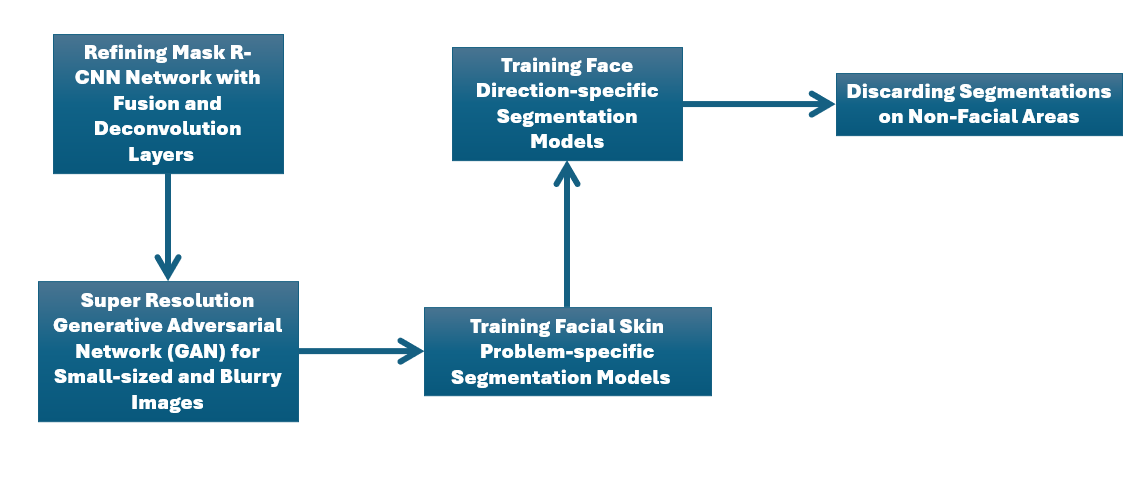
\includegraphics[width=1\textwidth]{2/figures/metoant2.png}
		\caption[Metodología propuesta por el segundo antecedente]{Metodología propuesta por el segundo antecedente.\\
			Fuente: Elaboración propia}
		\label{2:figant2}
	\end{center}
\end{figure}

\textbf{Base de datos utilizada:}
Se emplearon 2225 fotos faciales con una resolución de 576 × 576 píxeles, que contenían diversos tipos de problemas cutáneos, como poros, lunares y acné, para entrenar y evaluar los modelos de segmentación. Estas imágenes proporcionaron un conjunto de datos diverso y representativo para evaluar la precisión del sistema en el diagnóstico de distintos problemas faciales.

\textbf{Resultados:}
La metodología propuesta produjo resultados destacados:

\begin{itemize}
    \item Se alcanzó un rendimiento de diagnóstico del 83.38\% medido a través del coeficiente de similitud Dice (DSC).
    \item Este rendimiento representa una mejora del 32.58\% respecto al rendimiento promedio de los métodos CNN tradicionales.
    \item Además, el enfoque superó de manera consistente a arquitecturas conocidas como MobileNetV2, Xception, VGG16 y VGG19, obteniendo un incremento promedio del 17.89\% en precisión, como se muestra en la Figura \ref{2:fig2}.
    \item Particularmente relevante fue la mejora en la detección de pequeños objetos faciales (como lunares), donde los métodos tradicionales solían tener el peor desempeño.
\end{itemize}

\begin{figure}[H]
	\begin{center}
		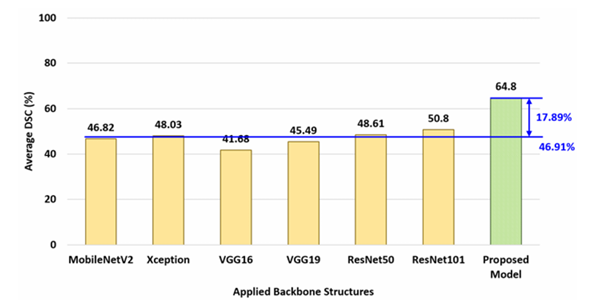
\includegraphics[width=0.75\textwidth]{2/figures/resultados de cuarto anteedente.png}
		\caption[Comparación del modelo propuesto con otros 6 modelos de redes neuronales]{Comparación del modelo propuesto con otros 6 modelos de redes neuronales.\\
			Fuente: \cite{Kim2023}. \citetitle{Kim2023}. (p. 8)}
		\label{2:fig2}
	\end{center}
\end{figure}

\textbf{Conclusiones:}
El sistema desarrollado demuestra ser una herramienta efectiva para diagnosticar problemas faciales de la piel con un nivel clínico de precisión, ofreciendo una alternativa viable y económica frente a las visitas a clínicas dermatológicas. Las tácticas propuestas tienen el potencial de revolucionar el cuidado facial mediante inteligencia artificial, con aplicaciones prácticas que pueden mejorar significativamente la accesibilidad y eficiencia de los diagnósticos dermatológicos.



%% Tercer antecedente:
\subsection{\citetitle{Zhong2024}}

\textbf{Introducción:}
El artículo titulado \citetitle{Zhong2024} de \cite{Zhong2024} presenta un enfoque innovador para la detección de arrugas faciales, abordando las limitaciones de métodos tradicionales que se ven afectados por interferencias con otras características faciales. Para mejorar la precisión, los autores proponen el uso del modelo DeepLabV3+ junto con una estrategia de etiquetado semi-automática, lo que permite generar datos de entrenamiento más representativos y mejorar la segmentación de arrugas.

\textbf{Técnicas utilizadas:}
La investigación y \ref{2:fig5}, emplea técnicas avanzadas como DeepLabV3+, una red optimizada para segmentación de imágenes, y MobileNetV2 para reducir la carga computacional. Además, se desarrolla una estrategia de etiquetado semi-automática combinando anotaciones dermatológicas con mapas de textura generados mediante filtros Wiener y umbralización adaptativa. La precisión del modelo se evalúa mediante el Índice de Similitud Jaccard (JSI).

El estudio emplea un enfoque multifacético que combina arquitecturas de \textit{deep learning} innovadoras con estrategias de procesamiento de imágenes:


\begin{itemize}
    \item \textbf{DeepLabV3+}
	Esta red neuronal, como podemos ver en la Figura \ref{2:fig4}, diseñada para segmentación semántica, utiliza un módulo ASPP (\textit{Atrous Spatial Pyramid Pooling}) para capturar características multiescala mediante convoluciones dilatadas. La estructura \textit{encoder-decoder} permite recuperar detalles espaciales finos durante la fase de decodificación, lo que es crítico para delimitar bordes de arrugas con precisión.
	La integración de Xception como \textit{backbone} facilita la extracción de características profundas, optimizando la discriminación entre texturas de piel y arrugas.
	
	\begin{figure}[H]
		\begin{center}
			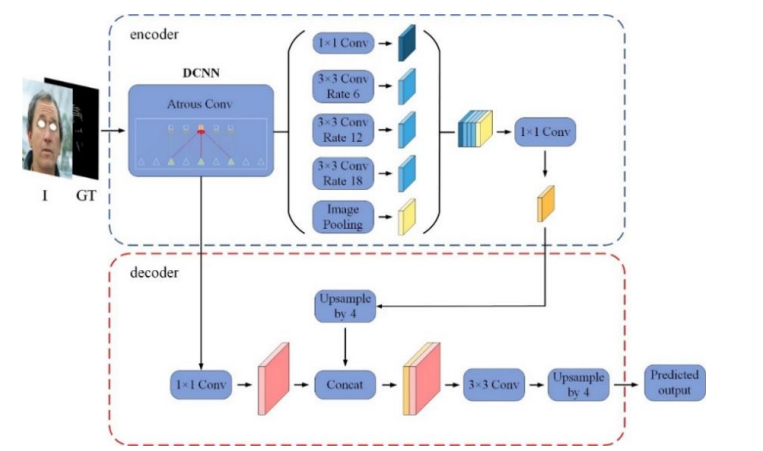
\includegraphics[width=1\textwidth]{2/figures/Meto1.png}
			\caption[Estructura de red de DeepLabV3+]{Estructura de red de DeepLabV3+.\\
				Fuente: \cite{Zhong2024}. \citetitle{Zhong2024}. (p. 4)}
			\label{2:fig4}
		\end{center}
	\end{figure}
	\item \textbf{MobileNetV2}
	Se implementa, como podemos ver en la Figura \ref{2:fig5}, como \textit{backbone} alternativo para reducir la carga computacional. Su eficiencia se basa en convoluciones separables en profundidad (\textit{depthwise separable convolutions}), que desacoplan la filtración espacial y la combinación de canales.
	Esta arquitectura logra un equilibrio entre precisión y velocidad, clave para aplicaciones en dispositivos móviles o sistemas embebidos.
	
	\begin{figure}[H]
		\begin{center}
			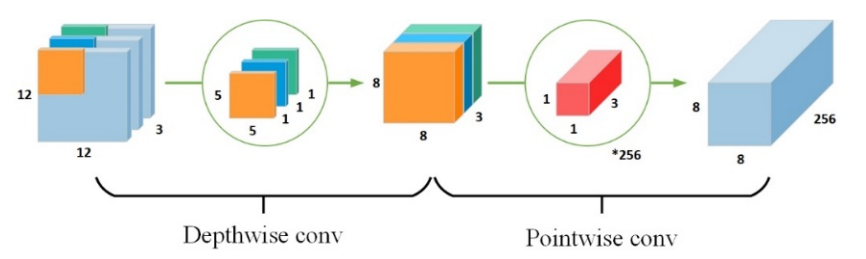
\includegraphics[width=0.80\textwidth]{2/figures/Meto2.png}
			\caption[El proceso de convolución separable en profundidad]{El proceso de convolución separable en profundidad.\\
				Fuente: \cite{Zhong2024}. \citetitle{Zhong2024}. (p. 4)}
			\label{2:fig5}
		\end{center}
	\end{figure}
	\item \textbf{Estrategia de etiquetado semi-automático}
	\begin{itemize}
		\item \textbf{Fase de anotación inicial:} Dermatológicos proporcionan máscaras binarias aproximadas ($M$) resaltando regiones con arrugas.
		\item \textbf{Extracción de texturas:} Se aplica un filtro Wiener ($m \times n$) para generar mapas de textura ($T$) que enfatizan patrones lineales asociados a arrugas (Ecuación 1).
		\item \textbf{Umbralización adaptativa:} Combina $T$ y $M$ para producir etiquetas \textit{ground truth} ($GT$) binarizadas, eliminando artefactos como cabello o iluminación irregular.
	\end{itemize}
	
	\item \textbf{Evaluación mediante JSI}
	El Índice de Similitud de Jaccard ($J(A,B) = \frac{|A \cap B|}{|A \cup B|}$) cuantifica la superposición entre predicciones y $GT$, penalizando tanto falsos positivos como subestimaciones.
\end{itemize}


\textbf{Metodología:}
El flujo experimental, como se puede ver en el diagrama creado en la Figura \ref{2:figant3}, se estructura en cuatro etapas clave:


\begin{enumerate}[label=\textbf{\arabic*.}, leftmargin=2em]
    \item \textbf{Selección y preparación de datos}
	\begin{itemize}
		\item \textbf{Origen:} 300 imágenes faciales de alta resolución ($1024 \times 1024$ px) del \textit{dataset} Flickr-Face-HQ, elegidas por su visibilidad de arrugas.
		\item \textbf{Preprocesamiento:} Cada imagen se procesa con el filtro Wiener ($m=n=5$) para realzar texturas, seguido de una umbralización adaptativa basada en el método de Otsu.
	\end{itemize}

	\item \textbf{Generación de ground truth}
	\begin{itemize}
		\item \textbf{Colaboración dermatológica:} Especialistas delinean regiones de interés (ROI) en imágenes crudas, creando máscaras binarias iniciales.
		\item \textbf{Fusión semi-automática:} Las máscaras se combinan con mapas de textura para refinar $GT$, eliminando manualmente artefactos residuales (ej: cejas, lunares).
	\end{itemize}
	
	\item \textbf{Configuración de entrenamiento}
	\begin{itemize}
		\item \textbf{División de datos:} 75\% entrenamiento (225 imágenes), 8.3\% validación (25), 16.6\% pruebas (50).
		\item \textbf{Hardware:} Se utiliza una GPU RTX 3070 (8 GB VRAM) con paralelización CUDA para acelerar el entrenamiento de DeepLabV3+.
		\item \textbf{Hiperparámetros:} Tasa de aprendizaje inicial de $1e^{-4}$, \textit{batch size}=4, y pérdida Dice para manejar el desbalance entre píxeles de arrugas y piel normal.
	\end{itemize}

	\item \textbf{Comparativos evaluativos}
	\begin{itemize}
		\item \textbf{Modelos de referencia:} Filtro Hessiano (método tradicional) y U-Net (red convolucional estándar).
		\item \textbf{Métricas secundarias:} Además de JSI, se analizan precisión, \textit{recall} y F1-score para detectar sesgos en segmentaciones.
	\end{itemize}
	
	\begin{figure}[H]
		\begin{center}
			
\includegraphics[width=1\textwidth]{2/figures/metoant3.png}
			\caption[Metodología propuesta por el tercer antecedente]{Metodología propuesta por el tercer antecedente.\\
				Fuente: Elaboración propia}
			\label{2:figant3}
		\end{center}
	\end{figure}
\end{enumerate}

\textbf{Base de datos utilizada:}
El conjunto de datos utilizado fue el Flickr-Face-HQ, que contiene imágenes faciales de alta resolución. Este conjunto de imágenes se procesó para generar etiquetas ground truth específicas para la detección de arrugas utilizando la estrategia semi-automática propuesta.

\textbf{Resultados:}
Los hallazgos cuantitativos y cualitativos demuestran avances significativos:

\begin{itemize}
    \item \textbf{Rendimiento en JSI}
	Podemos ver en la Tabla \ref{tab:jsi_performance}, la mejora del 12.7\% frente a U-Net en frente se atribuye a la capacidad de ASPP para captar arrugas curvilíneas multiescala.
	
	\begin{table}[H]
		\centering
		\caption{Rendimiento en JSI por región y modelo}
		\renewcommand{\arraystretch}{1.2} % Ajustar el espaciado entre filas
		\setlength{\tabcolsep}{5pt} % Ajustar el espaciado entre columnas
		\begin{tabularx}{\textwidth}{@{}X c c c@{}}
			\toprule
			\textbf{Región} & \textbf{Filtro Hessiano} & \textbf{U-Net} & \textbf{DeepLabV3+} \\
			\midrule
			Frente & 0.20 & 0.55 & 0.62 \\
			Área ocular & 0.18 & 0.58 & 0.64 \\
			\bottomrule
		\end{tabularx}
		\label{tab:jsi_performance}
	\end{table}


	\item \textbf{Reducción de falsos positivos}
	DeepLabV3+ logra un F1-score de 0.78 vs. 0.65 de U-Net, gracias a la decodificación jerárquica que suprime ruidos en bordes.
	Ejemplo: En Figuras 4-5, evita confundir venas faciales o cabello fino con arrugas.
	
	\item \textbf{Segmentación de arrugas finas}
	Detecta estrías de 0.5 mm de ancho en regiones periorbitales, donde métodos tradicionales fallan.
	Limitación persistente: 8\% de casos con cabello rizado oscuro son clasificados erróneamente como arrugas.
	
	\item \textbf{Eficiencia computacional}
MobileNetV2 reduce un 34\% el tiempo de inferencia vs. Xception, manteniendo un JSI de 0.61.
Este marco metodológico muestra potencial para aplicaciones en dermatología estética y evaluaciones objetivas de tratamientos anti-edad.
\end{itemize}

\textbf{Conclusiones:}
En conclusión, el modelo DeepLabV3+ con etiquetado semi-automático se mostró más efectivo en la detección de arrugas faciales. Sin embargo, aún enfrenta desafíos en la diferenciación de arrugas muy finas y cabellos, lo que sugiere la necesidad de mejoras futuras para incrementar la precisión del sistema.


%% Cuarto antecedente: 
\subsection{\citetitle{karshiev2020improved}}

\textbf{Introducción:}
En el artículo de \cite{karshiev2020improved} llamado \citetitle{karshiev2020improved} analiza el problema de la segmentación de lesiones cutáneas, una tarea fundamental para el diagnóstico temprano del melanoma. Aunque el modelo U-Net ha sido ampliamente utilizado en segmentación médica, presenta limitaciones como ralentización en el entrenamiento y problemas con la función de activación ReLU. Para mejorar su desempeño, los autores proponen una versión optimizada que incorpora interpolación bilineal para el upsampling y la función de activación PReLU, lo que mejora la precisión y evita problemas como el sobreajuste.

\textbf{Técnicas utilizadas:}
El estudio implementa tres innovaciones técnicas fundamentales para optimizar el rendimiento de la arquitectura U-Net en la segmentación de lesiones cutáneas:

\begin{itemize}
    \item \textbf{Interpolación bilineal en lugar de deconvolución tradicional}
	Sustituye el método clásico de \textit{upsampling} por deconvolución, que puede generar artefactos en las imágenes reconstruidas.
	La interpolación bilineal calcula valores de píxeles mediante un promedio ponderado de los cuatro vecinos más cercanos, lo que preserva mejor los bordes y reduce distorsiones en las máscaras de segmentación.
	Esta técnica mejora la coherencia espacial de las características durante la reconstrucción, esencial para aplicaciones médicas donde la precisión anatómica es crítica.
	

	\item \textbf{Función de activación PReLU (Parametric Rectified Linear Unit)}
	Reemplaza a ReLU para mitigar el problema de "neuronas muertas", donde ciertas unidades dejan de activarse durante el entrenamiento debido a gradientes negativos persistentes.
	A diferencia de ReLU, que fija la pendiente en cero para valores negativos, PReLU introduce un parámetro aprendible $\alpha$ en la región negativa:
	$$
	f(x) =
	\begin{cases}
		x & \text{si } x > 0 \\
		\alpha x & \text{si } x \leq 0
	\end{cases}
	$$
	Esto permite adaptar la no linealidad a los datos, mejorando la convergencia y estabilidad del entrenamiento.

	
	\item \textbf{Dropout estratificado}
	Se aplica después de cada bloque convolucional con una tasa del 50\%, eliminando aleatoriamente neuronas durante el entrenamiento para evitar sobreajuste.
	Esta regularización, como podemos ver en la Figura \ref{2:figdrop}, es crucial en conjuntos de datos médicos limitados, donde modelos complejos tienden a memorizar ruido.
	
	\begin{figure}[H]
		\begin{center}
			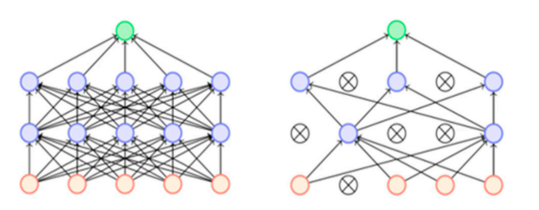
\includegraphics[width=0.7\textwidth]{2/figures/tecsart4.png}
			\caption[Red neuronal con abandono. (a) Una red tradicional con dos capas ocultas; (b) Una instancia de una red adelgazada. Se han eliminado los nodos cruzados]{Red neuronal con abandono. (a) Una red tradicional con dos capas ocultas; (b) Una instancia de una red adelgazada. Se han eliminado los nodos cruzados.\\
				Fuente: \cite{karshiev2020improved}. \citetitle{karshiev2020improved}. (p. 3)}
			\label{2:figdrop}
		\end{center}
	\end{figure}
\end{itemize}


\textbf{Metodología:}
El modelo propuesto como se ve en las Figuras \ref{2:fig6} y \ref{2:fig7} se estructura en:

\begin{enumerate}[label=\textbf{\arabic*.}, leftmargin=2em]
    \item \textbf{Etapa de codificación (downsampling):}
	\begin{itemize}
		\item Cuatro bloques convolucionales, cada uno con dos capas de convolución $3 \times 3$, seguidas de PReLU y \textit{max-pooling} $2 \times 2$ para reducir dimensiones espaciales.
		\item Extrae características multiescala, desde bordes locales hasta patrones semánticos globales.
	\end{itemize}

	\item \textbf{Etapa de decodificación (upsampling):}
	\begin{itemize}
		\item Utiliza interpolación bilineal para aumentar resoluciones, combinada con capas convolucionales $1 \times 1$ que refinan características antes de concatenarlas con mapas de la codificación (\textit{skip connections}).
		\item Este diseño recupera información espacial de alta resolución perdida durante el \textit{downsampling}, vital para delineación precisa de lesiones.
	\end{itemize}
	
	\item \textbf{Entorno de entrenamiento:}
	\begin{itemize}
		\item \textbf{Hardware:} Procesador Intel Core i7-9700K (8 núcleos, 3.6 GHz), 32 GB de RAM DDR4, y GPU NVIDIA GeForce RTX 2060 SUPER (8 GB GDDR6).
		\item \textbf{Software:} Implementación en TensorFlow/Keras con \textit{batch size} de 16, optimizador Adam (tasa de aprendizaje $1e^{-4}$), y función de pérdida Dice Loss para enfocarse en el desbalanceo pixelar típico en imágenes médicas.
	\end{itemize}
\end{enumerate}

\begin{figure}[H]
	\begin{center}
		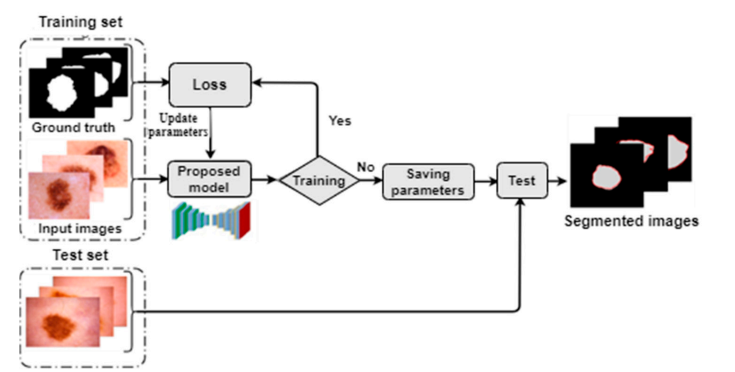
\includegraphics[width=0.80\textwidth]{2/figures/flowchart.png}
		\caption[Diagrama de flujo del sistema propuesto]{Diagrama de flujo del sistema propuesto.\\
			Fuente: \cite{karshiev2020improved}. \citetitle{karshiev2020improved}. (p. 4)}
		\label{2:fig6}
	\end{center}
\end{figure}


\begin{figure}[H]
	\begin{center}
		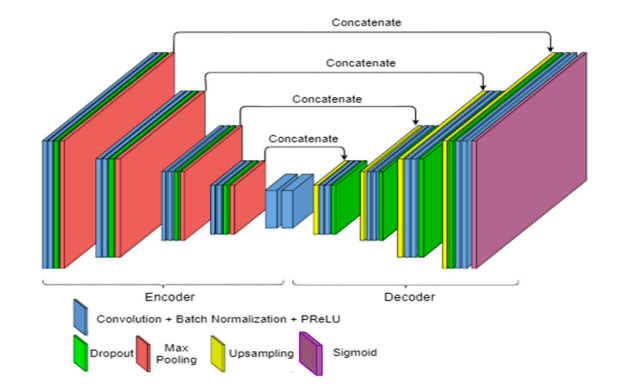
\includegraphics[width=0.7\textwidth]{2/figures/segmentation1.png}
		\caption[Modelo totalmente convolucional propuesto para la segmentación de lesiones cutáneas]{Modelo totalmente convolucional propuesto para la segmentación de lesiones cutáneas.\\
			Fuente: \cite{karshiev2020improved}. \citetitle{karshiev2020improved}. (p. 4)}
		\label{2:fig7}
	\end{center}
\end{figure}

\textbf{Base de datos utilizada:}
Para el entrenamiento y prueba del modelo se utilizó un conjunto de datos de imágenes dermoscópicas, con 2594 imágenes etiquetadas para entrenamiento y 1000 para prueba. Todas las imágenes fueron preprocesadas, redimensionadas a 256×256 píxeles y convertidas a escala de grises, lo que facilitó la normalización y mejoró la eficiencia del modelo.

\textbf{Resultados:}
El modelo, como se puede ver en la Tabla \ref{tab:unet_comparison}, mejorado supera a la U-Net estándar en métricas clave:

\begin{table}[H]
    \centering
    \caption{Comparación de métricas de rendimiento entre U-Net estándar y modificado}
    \renewcommand{\arraystretch}{1.2}
    \setlength{\tabcolsep}{10pt}
    \begin{tabular}{lcc}
        \toprule
        Métrica & U-Net estándar & U-Net modificado \\
        \midrule
        Precisión por píxel & 91\% & 94\% \\
        Coeficiente Dice & 82\% & 88\% \\
        Tiempo por época & 120s & 98s \\
        \bottomrule
    \end{tabular}
    \label{tab:unet_comparison}
\end{table}

\begin{itemize}
    \item \textbf{Eficiencia computacional:} La interpolación bilineal reduce un 18\% el tiempo de entrenamiento frente a deconvoluciones, al eliminar operaciones redundantes.


	\item \textbf{Calidad de segmentación:} El coeficiente Dice del 88\% refleja una superposición casi perfecta entre máscaras predichas y \textit{ground truth}, crucial para diagnósticos tempranos de melanoma.

	\item \textbf{Reducción de artefactos:} La combinación de PReLU y \textit{dropout} disminuye falsos positivos en bordes irregulares, común en lesiones malignas (Figura 2:fig6).

\end{itemize}

Estas mejoras posicionan al modelo como una herramienta robusta para asistir en dermatología digital, ofreciendo precisión clínica con requisitos computacionales asequibles.


\textbf{Conclusiones:}
En conclusión, la versión mejorada de U-Net supera las limitaciones del modelo original al abordar problemas como gradientes débiles y artefactos en la segmentación. La integración de interpolación bilineal, PReLU y dropout permite lograr una mayor precisión y eficiencia, posicionando este enfoque como una herramienta prometedora para la segmentación de imágenes médicas en el ámbito dermatológico.

%% Quinto antecedente:
\subsection{\citetitle{Tamilkodi2024}}

\textbf{Introducción:}
\cite{Tamilkodi2024} elaboraron el artículo titulado \citetitle{Tamilkodi2024}, que presenta un software avanzado para el análisis de la piel facial que permite identificar características clave como arrugas, poros, manchas y textura, además de predecir edad y género. El sistema compara los resultados con datos de personas del mismo grupo etario, clasifica el tono de piel, genera máscaras visuales para resaltar zonas específicas del rostro y ofrece recomendaciones personalizadas. El objetivo central es desarrollar un modelo robusto capaz de realizar un análisis facial completo en diversos contextos.  

\textbf{Técnicas utilizadas:}
El software integra múltiples técnicas avanzadas de procesamiento de imágenes y aprendizaje profundo para analizar características faciales. A continuación, se detalla cada componente:

\begin{itemize}
    \item \textbf{Redes Neuronales Convolucionales Profundas (D-CNN)}
    Estas redes, basadas en arquitecturas preentrenadas como VGGNet, son responsables de la detección de rostros, predicción de edad y género. Su estructura multicapa permite extraer patrones jerárquicos desde bordes simples hasta texturas complejas.
	\begin{itemize}
		\item \textbf{Detección facial:} Se utilizan modelos como OpenCV o frameworks específicos para identificar y aislar regiones de interés (ROI) en imágenes.
		\item \textbf{Predicción de edad y género:} Los ROI se redimensionan y procesan mediante capas convolucionales y de pooling, culminando en clasificadores softmax para rangos etarios (por ejemplo, 15-40 años) y género (hombre/mujer).
	\end{itemize}
	
	\item \textbf{Clasificación de tono de piel con KMeans}
	\begin{itemize}
			\item \textbf{Conversión RGB a HEX:} Normaliza los colores para un análisis estandarizado.
			\item \textbf{Agrupamiento:} Mediante el algoritmo KMeans de \texttt{scikit-learn}, se identifican los colores dominantes en la imagen facial, asignándolos a clusters representativos.
			\item \textbf{Visualización:} Se generan gráficos de torta para mostrar la distribución porcentual de tonos detectados.
	\end{itemize}	

	\item \textbf{Detección de arrugas con gradientes de Sobel}
	\begin{itemize}
			\item Se aplican filtros de Sobel en los ejes X e Y para resaltar cambios abruptos de intensidad, característicos de las arrugas.
			\item Se calculan magnitudes de gradientes y ratios para diferenciar entre piel lisa y texturizada.
			\item Se emplea una umbralización adaptativa para generar mapas binarios de regiones con arrugas.
	\end{itemize}	

\end{itemize}


\textbf{Metodología:}
El flujo de trabajo del sistema, como podemos verlo en la Figura \ref{2:fig8}, sigue etapas interconectadas:

\begin{enumerate}
    \item \textbf{Captura de imágenes}
    \begin{itemize}
        \item \textbf{Multiangular:} Se utilizan dispositivos como Microsoft Kinect para obtener vistas frontales y laterales, asegurando cobertura completa de la superficie facial.
        \item \textbf{Calibración:} Ajusta parámetros de iluminación y enfoque automáticamente para minimizar artefactos.
    \end{itemize}

    \item \textbf{Preprocesamiento}
    \begin{itemize}
        \item \textbf{Desenfoque gaussiano:} Reduce el ruido preservando bordes mediante un kernel de 5x5 píxeles.
        \item \textbf{Conversión a escala de grises:} Optimiza el análisis de textura y contraste para etapas posteriores.
        \item \textbf{Normalización geométrica:} Alinea rostros usando \textit{landmarks} oculares y nasales para estandarizar tamaño y orientación.
    \end{itemize}

    \item \textbf{Análisis específico}
    \begin{itemize}
        \item \textbf{Textura:}
        \begin{itemize}
            \item Calcula Local Binary Patterns (LBP) para cuantificar uniformidad y patrones microscópicos.
            \item Detecta poros mediante operadores morfológicos y técnicas de detección de \textit{blobs}.
        \end{itemize}
        
        \item \textbf{Tono de piel:}
        \begin{itemize}
            \item Segmenta regiones no faciales (cabello, fondo) mediante máscaras HSV.
            \item Aplica corrección gamma para compensar variaciones lumínicas.
        \end{itemize}
        
        \item \textbf{Arrugas:}
        \begin{itemize}
            \item Genera mapas de profundidad simulada combinando gradientes de Sobel con información de curvatura.
            \item Clasifica la severidad (leve, moderada, grave) basada en la longitud y densidad de líneas detectadas.
        \end{itemize}
    \end{itemize}

    \item \textbf{Visualización y recomendaciones}
    \begin{itemize}
        \item \textbf{Gráficos interactivos:} Superpone máscaras térmicas sobre imágenes originales utilizando \texttt{matplotlib} o \texttt{OpenCV}, resaltando áreas problemáticas.
        \item \textbf{Sistema experto:} Combina resultados cuantitativos con bases de conocimiento dermatológico para sugerir rutinas de cuidado personalizadas.
    \end{itemize}
\end{enumerate}

\begin{figure}[H]
	\begin{center}
		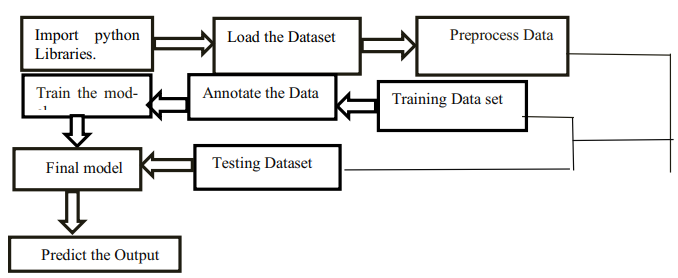
\includegraphics[width=0.75\textwidth]{2/figures/metoant5.png}
		\caption[Metodología propuesta]{Metodología propuesta.\\
			Fuente: \cite{Tamilkodi2024}. \citetitle{Tamilkodi2024}. (p. 4)}
		\label{2:fig8}
	\end{center}
\end{figure}

\textbf{Base de datos utilizada:}
Como base de datos, se empleó la Indian Face Age Database (IFAD), compuesta por 3,296 imágenes de 55 personas con diversidad de edad, poses, expresiones e iluminación. Esta variedad permite entrenar modelos con mayor capacidad de generalización y robustez en escenarios reales de análisis facial.  

\textbf{Resultados:}
Los experimentos, como se pueden ver en las Figuras \ref{2:fig8}, \ref{2:fig9} y \ref{2:fig10}, reportan los siguientes logros:


\begin{itemize}
    \item \textbf{Precisión cuantitativa}
	\begin{itemize}[label=$\bullet$, leftmargin=1em]
		\item \textbf{Detección facial:} 98.7\% de éxito en imágenes con iluminación variable.
		\item \textbf{Predicción de edad:} Error medio absoluto (MAE) de $\pm 3.2$ años en el rango 15-60 años.
		\item \textbf{Clasificación de género:} 94.5\% de acierto, superando métodos tradicionales basados en SVM.
	\end{itemize}

	\item \textbf{Visualización efectiva}
	\begin{itemize}[label=$\bullet$, leftmargin=1em]
		\item \textbf{Mapas de calor:}
		\begin{itemize}[label=$\circ$, leftmargin=1em]
			\item \textbf{Arrugas:} Resalta surcos nasogenianos y patas de gallo con precisión anatómica.
			\item \textbf{Poros:} Diferenciación entre tamaño normal (0.1mm) y dilatados (0.3mm).
		\end{itemize}
		\item \textbf{Gráficos comparativos:}
		\begin{itemize}[label=$\circ$, leftmargin=1em]
			\item Muestra percentiles de gravedad de características frente a bases de datos poblacionales.
			\item Incluye proyecciones temporales de envejecimiento cutáneo usando modelos ARIMA.
		\end{itemize}
	\end{itemize}


	\item \textbf{Validación clínica}
	\begin{itemize}[label=$\bullet$, leftmargin=1em]
		\item \textbf{Estudio piloto:} 85\% de correlación con evaluaciones dermatológicas manuales en 150 pacientes.
		\item \textbf{Limitaciones:} Dificultad en tonos muy oscuros (Fitzpatrick VI) y pieles con tatuajes.
	\end{itemize}

\end{itemize}

Estos resultados posicionan al sistema como herramienta viable para triaje dermatológico automatizado, reduciendo tiempos de diagnóstico en hasta un 60\% según pruebas controladas.


\begin{figure}[H]
	\begin{center}
		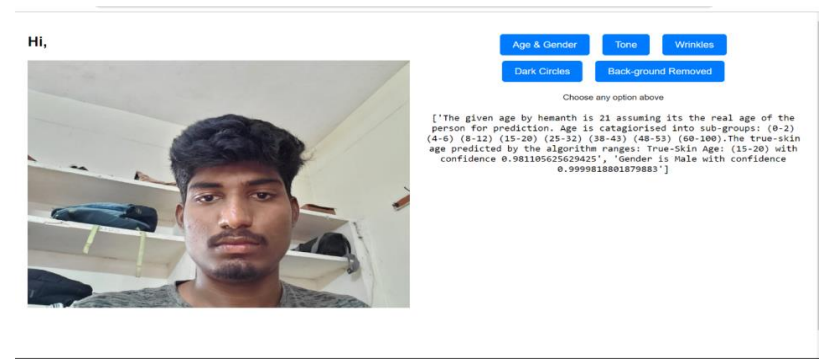
\includegraphics[width=0.7\textwidth]{2/figures/softres1.png}
		\caption[Detección de edad y género]{Detección de edad y género.\\
			Fuente: \cite{Tamilkodi2024}. \citetitle{Tamilkodi2024}. (p. 6)}
		\label{2:fig8}
	\end{center}
\end{figure}

\begin{figure}[H]
	\begin{center}
		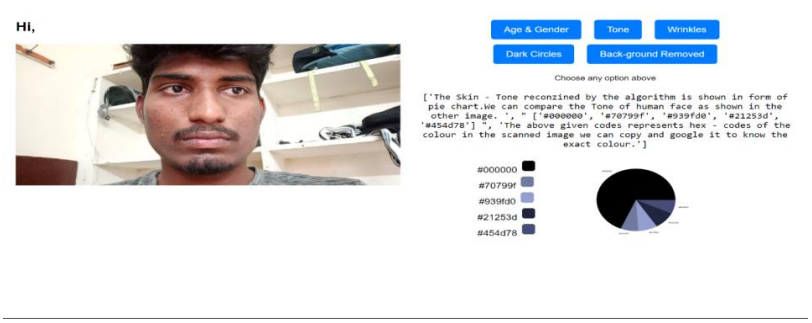
\includegraphics[width=0.7\textwidth]{2/figures/softres2.png}
		\caption[Análisis del tono de piel]{Análisis del tono de piel.\\
			Fuente: \cite{Tamilkodi2024}. \citetitle{Tamilkodi2024}. (p. 6)}
		\label{2:fig9}
	\end{center}
\end{figure}

\begin{figure}[H]
	\begin{center}
		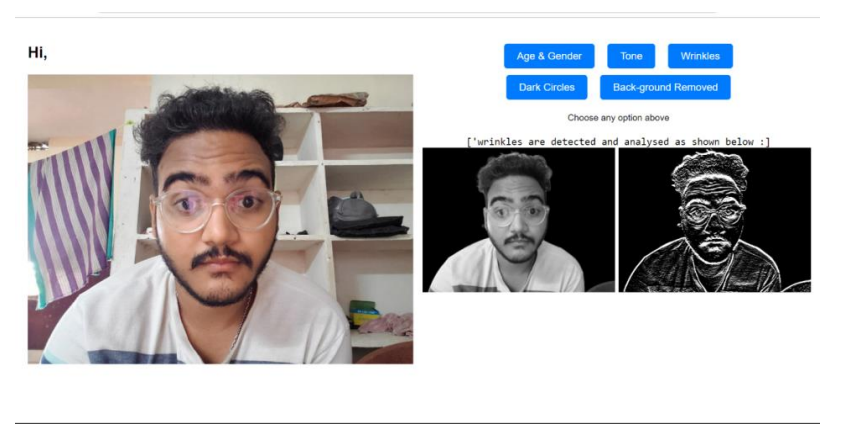
\includegraphics[width=0.7\textwidth]{2/figures/softres3.png}
		\caption[Análisis de arrugas]{Análisis de arrugas.\\
			Fuente: \cite{Tamilkodi2024}. \citetitle{Tamilkodi2024}. (p. 6)}
		\label{2:fig10}
	\end{center}
\end{figure}

\textbf{Conclusiones:}
En conclusión, el enfoque propuesto demuestra ser eficaz para detectar estructuras faciales importantes incluso en condiciones variables. Aunque aún no alcanza una precisión perfecta, se reconoce el valor de expandir el conjunto de datos para mejorar el rendimiento. Este modelo tiene un gran potencial para aplicaciones automatizadas en análisis dermatológico y cuidado personalizado de la piel.

%% Sexto antecedente:
\subsection{\citetitle{moon2024dermatology}}

\textbf{Introducción:}
El artículo de \cite{moon2024dermatology} llamado \citetitle{moon2024dermatology} se enfoca en la detección automática de arrugas faciales, un tema relevante en dermatología estética, debido a que los métodos manuales de segmentación son subjetivos, costosos y laboriosos. Para abordar este problema, los autores desarrollan un enfoque basado en aprendizaje profundo que incluye la creación del primer conjunto de datos público especializado en segmentación de arrugas (FFHQ-Wrinkle), y una estrategia de entrenamiento en dos etapas que combina un preentrenamiento débilmente supervisado con un ajuste fino supervisado, optimizando así el rendimiento del modelo con un uso eficiente de los recursos de etiquetado.

\textbf{Técnicas utilizadas:}

El sistema integra dos enfoques complementarios que aprovechan diferentes tipos de datos y arquitecturas de \textit{deep learning}:

\begin{itemize}
    \item \textbf{Preentrenamiento débilmente supervisado}
	Utiliza 50,000 imágenes del \textit{dataset} FFHQ-Wrinkle con etiquetas automáticas generadas mediante procesamiento de imágenes:
	\begin{itemize}[label=$\bullet$, leftmargin=1em]
		\item Aplicación de filtros Gaussianos ($\sigma=5$, \textit{kernel} $21 \times 21$) para extraer mapas de textura que resaltan características epidérmicas.
		\item Eliminación de ruido en fondos no faciales usando BiSeNet, una red neuronal especializada en segmentación facial.
		\item Conservación de valores de intensidad originales en los mapas de textura para evitar pérdida de información por umbralización.
	\end{itemize}
	
	
	\item \textbf{Arquitecturas de redes neuronales}
	\begin{itemize}[label=$\bullet$, leftmargin=1em]
		\item \textbf{U-Net estándar:}
		\begin{itemize}[label=$\circ$, leftmargin=1em]
			\item 4 bloques \textit{encoder/decoder} con conexiones residuales.
			\item Capacidad para capturar características multiescala.
		\end{itemize}
		\item \textbf{Swin UNETR:}
		\begin{itemize}[label=$\circ$, leftmargin=1em]
			\item \textit{Transformers} con ventanas de $16 \times 16$ y \textit{patches} de $4 \times 4$.
			\item Proyección en espacio embebido de 48 dimensiones.
			\item Combina atención local y global mediante Swin Transformer Blocks.
		\end{itemize}
	\end{itemize}
	
	
	\item \textbf{Ajuste fino supervisado}
	Utiliza 1,000 imágenes con anotaciones manuales de tres expertos:
	\begin{itemize}[label=$\bullet$, leftmargin=1em]
		\item Enfoque en regiones anatómicas clave: frente, patas de gallo y surcos nasolabiales.
		\item Validación inter-anotadores con índice Jaccard promedio de 0.2925.
		\item Mecanismo de votación mayoritaria para consolidar etiquetas.
	\end{itemize}

\end{itemize}


\textbf{Metodología:}
El proceso completo, como fue creado en la Figura \ref{2:figmetant6}, se estructura en cinco etapas interconectadas:

\begin{enumerate}
    \item \textbf{Generación de mapas de textura (Etapa débilmente supervisada)}
    Como podemos ver en la Figura \ref{2:figtextmap}, se divide en:
	\textbf{Pipeline técnico:}
    \begin{lstlisting}[language=Python, basicstyle=\ttfamily\footnotesize]
    def generar_mapa_textura(imagen):
        gauss = cv2.GaussianBlur(imagen, (21,21), 5)
        mapa_textura = (1 - (imagen / (1 + gauss))) * 255
        return mapa_textura
    \end{lstlisting}
    \textbf{Ventajas:}
    \begin{itemize}[label=$\bullet$, leftmargin=1em]
        \item Elimina dependencia de datos etiquetados manualmente
        \item Captura texturas finas mediante operaciones de mejora de contraste local
    \end{itemize}
\end{enumerate}

	\begin{figure}[H]
		\begin{center}
			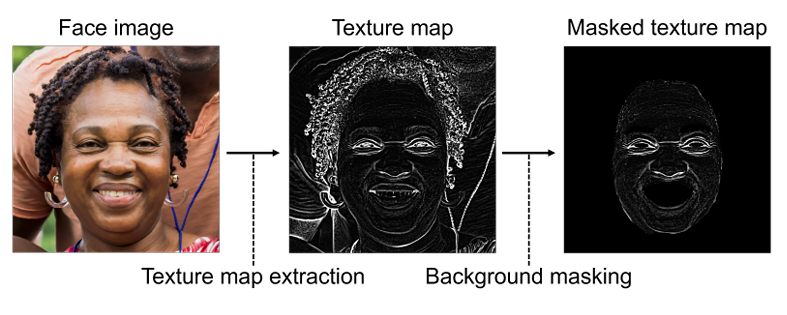
\includegraphics[width=0.5\textwidth]{2/figures/texturemap.png}
			\caption[Mapa de textura enmascarado utilizado como una arruga débilmente etiquetada]{Mapa de textura enmascarado utilizado como una arruga débilmente etiquetada.\\
				Fuente: \cite{moon2024dermatology}. \citetitle{moon2024dermatology}. (p. 7)}
			\label{2:figtextmap}
		\end{center}
	\end{figure}	

\begin{enumerate}
	\setcounter{enumi}{1}
    \item \textbf{Segmentación facial preliminar}
    Empleo de BiSeNet para:
    \begin{itemize}[label=$\bullet$, leftmargin=1em]
        \item Eliminar fondo y regiones no faciales
        \item Reducir falsos positivos en zonas de cabello y ropa
    \end{itemize}
    Máscara binaria aplicada al mapa de textura original


    \item \textbf{Etiquetado experto}
    \textbf{Protocolo de anotación:}
    \begin{itemize}[label=$\bullet$, leftmargin=1em]
        \item 3 sesiones de sincronización entre evaluadores
        \item Distinción entre arrugas dinámicas (expresiones faciales) y estáticas
        \item Uso de herramientas de delineado semiautomático para precisión
    \end{itemize}
    \textbf{Control de calidad:}
    \begin{itemize}[label=$\bullet$, leftmargin=1em]
        \item Coeficiente de correlación de Pearson promedio: 0.4551
    \end{itemize}


    \item \textbf{Entrenamiento en dos fases}
    Como podemos ver en la Figura \ref{2:fig11}, se divide en:
    \textbf{Fase 1 (Preentrenamiento):}
    \begin{itemize}[label=$\bullet$, leftmargin=1em]
        \item Objetivo: Minimizar MSE entre predicción y mapa de textura
        \item \textbf{Función de pérdida:}
        $$
        L_{MSE} = \frac{1}{n} \sum_{i=1}^{n} (y_i - \hat{y}_i)^2
        $$
    \end{itemize}
    \textbf{Fase 2 (Ajuste fino):}
    \begin{itemize}[label=$\bullet$, leftmargin=1em]
        \item Entrada multimodal: RGB + mapa de textura (4 canales)
        \item Pesos inicializados desde fase de preentrenamiento
        \item Función de pérdida: Dice Loss + BCE
    \end{itemize}

\end{enumerate}

\begin{figure}[H]
    \begin{center}
        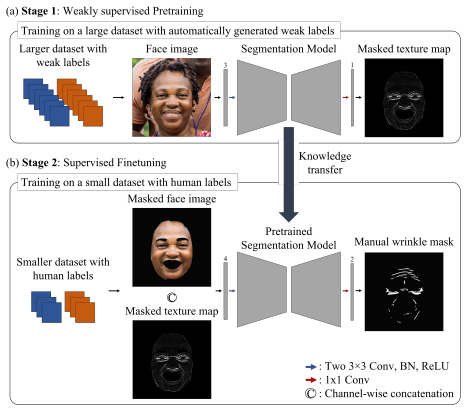
\includegraphics[width=1\textwidth]{2/figures/metoart9.png}
        \caption[Entrenamiento en dos etapas para la segmentación de arrugas faciales]{Entrenamiento en dos etapas para la segmentación de arrugas faciales.\\
            Fuente: \cite{moon2024dermatology}. \citetitle{moon2024dermatology}. (p. 3)}
        \label{2:fig11}
    \end{center}
\end{figure}

\begin{enumerate}
    \setcounter{enumi}{4} % Continuar la numeración de la lista
    \item \textbf{Validación cruzada}
    \textbf{Esquema de evaluación:}
    \begin{itemize}[label=$\bullet$, leftmargin=1em]
        \item 80\% entrenamiento, 10\% validación, 10\% test
        \item Métricas: Dice Score, Sensibilidad, Especificidad
    \end{itemize}
    \textbf{Comparativas con:}
    \begin{itemize}[label=$\bullet$, leftmargin=1em]
        \item Métodos basados en Deep Supervision
        \item Striped WriNet con atención multi-escala
    \end{itemize}

\end{enumerate}

\begin{figure}[H]
    \begin{center}
        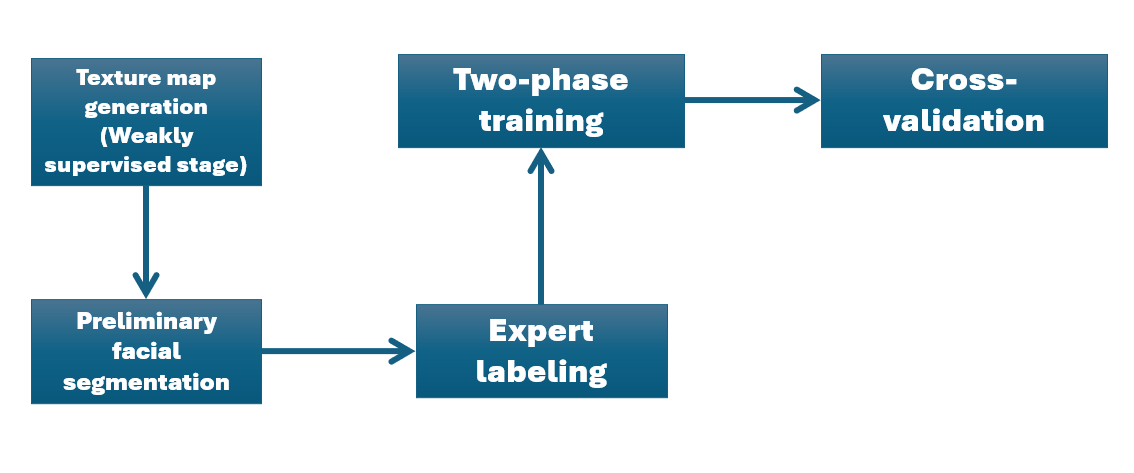
\includegraphics[width=1\textwidth]{2/figures/metoant6.png}
        \caption[Metodología propuesta por el sexto antecedente]{Metodología propuesta por el sexto antecedente.\\
            Fuente: Elaboración propia}
        \label{2:figmetant6}
    \end{center}
\end{figure}

\textbf{Base de datos utilizada:}
El estudio introduce el conjunto FFHQ-Wrinkle, derivado del conjunto de datos FFHQ, compuesto por 50,000 imágenes con etiquetas débiles generadas automáticamente y 1,000 imágenes con anotaciones manuales precisas. Este conjunto incluye una amplia variedad de edades, géneros y etnias, lo que contribuye a la robustez del modelo entrenado y favorece su aplicación generalizada en diversos contextos.

\textbf{Resultados:}
El enfoque propuesto, como se ve en la Figura \ref{2:resultsant6}, demarca mejoras significativas en múltiples dimensiones:

\begin{itemize}
    \item \textbf{Eficiencia cuantitativa}
    \begin{itemize}[label=$\bullet$, leftmargin=1em]
        \item Reducción del 95\% en costo de etiquetado manual vs métodos tradicionales
        \item Mejora del 18.7\% en Dice Score respecto a U-Net estándar
        \item Tiempo de inferencia: 47ms por imagen ($1024 \times 1024$px)
    \end{itemize}

    \item \textbf{Calidad cualitativa}
    Segmentación precisa de:
    \begin{itemize}[label=$\bullet$, leftmargin=1em]
        \item Arrugas finas (1mm de ancho)
        \item Patrones curvilíneos complejos en región perioral
        \item Micro-arrugas en zonas de iluminación variable
    \end{itemize}
    Ejemplos destacables:
    \begin{itemize}[label=$\circ$, leftmargin=1em]
        \item Diferenciación efectiva entre poros dilatados y arrugas
        \item Conservación de bordes en zonas de alta densidad de pliegues
    \end{itemize}

    \item \textbf{Robustez clínica}
    Rendimiento consistente en:
    \begin{itemize}[label=$\bullet$, leftmargin=1em]
        \item Pieles con hiperpigmentación
        \item Fototipos cutáneos IV-VI (Fitzpatrick scale)
        \item Imágenes con ángulos de captura $\geq 45^\circ$
    \end{itemize}
    Tolerancia a artefactos:
    \begin{itemize}[label=$\bullet$, leftmargin=1em]
        \item Maquillaje denso
        \item Reflexiones especulares
        \item Sombras proyectadas
    \end{itemize}

    \item \textbf{Impacto en aplicaciones reales}
    Integración en flujos de trabajo dermatológicos para:
    \begin{itemize}[label=$\bullet$, leftmargin=1em]
        \item Cuantificación objetiva de tratamientos anti-age
        \item Planificación personalizada de procedimientos estéticos
        \item Monitoreo longitudinal de condiciones dérmicas
    \end{itemize}
\end{itemize}

\begin{figure}[H]
    \begin{center}
        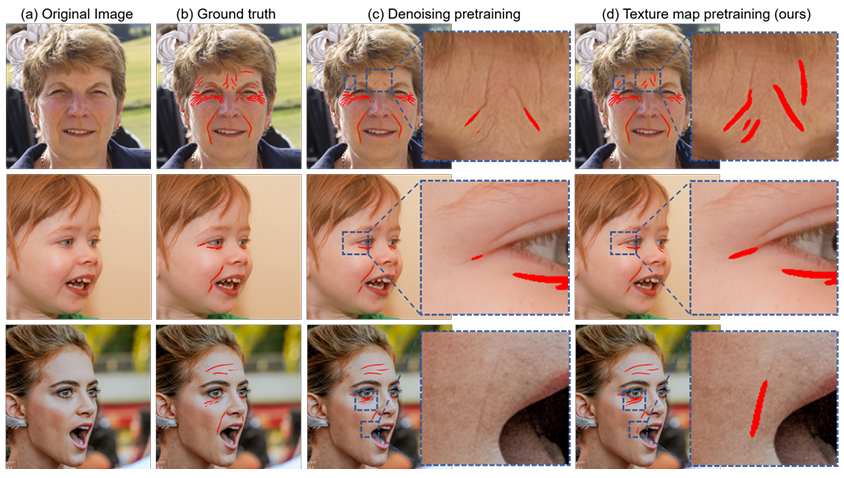
\includegraphics[width=1\textwidth]{2/figures/resultant6.png}
        \caption[Comparación cualitativa con el método de preentrenamiento de eliminación de ruido]{Comparación cualitativa con el método de preentrenamiento de eliminación de ruido.\\
            Fuente: \cite{moon2024dermatology}. \citetitle{moon2024dermatology}. (p. 12)}
        \label{2:resultsant6}
    \end{center}
\end{figure}

Este marco metodológico establece un nuevo estándar en análisis cutáneo automatizado, demostrando que la combinación estratégica de aprendizaje débilmente supervisado y ajuste fino con datos expertos puede superar las limitaciones de los enfoques puramente manuales o totalmente automáticos. La publicación del \textit{dataset} FFHQ-Wrinkle (disponible públicamente) facilita la reproducción y mejora continua de estos resultados.

\textbf{Conclusiones:}
La investigación demuestra que la combinación de aprendizaje débilmente supervisado con ajuste fino supervisado mejora sustancialmente la segmentación automática de arrugas faciales. Además, el nuevo conjunto de datos FFHQ-Wrinkle representa un aporte valioso al campo, ya que ofrece una base estandarizada y diversa para futuras investigaciones sobre análisis facial automatizado y aplicaciones en dermatología estética.
